\chapter{Electrohydrodynamics in microchannels}

In this chapter, the fundamental physics behind electrokinetic flow,
important for later discussions, will be presented. Particularly, a
modelling approach based on the coupling of Navier-Stokes,
Nernst-Planck and Poission's equations is given.

\section{Electrical double layers}
Consider an electrically neutral liquid, i.e. a liquid containing the
same amount of positive and negative ions. When this liquid is
introduced to, for example, a negatively charged surface, this even
charge distribution is disturbed in an area close to the surface. Due
to the introduced electrostatic forces, positive ions will be
attracted to the surface leaving a positive net charge in the vicinity
of the surface. It is possible to divide this positively charged
region in the liquid into two different layers. In the direct vicinity
of the surface, positive ions will adsorb onto the surface making them
less mobile than the others in the positively net charged area closer
to the bulk liquid. The two layers are often referred to as the Stern
layer (adsorbed) and the diffusive layer (mobile). This is also
illustrated in fig. \ref{fig:edl_charge} \cite{ren_book}

%potential charge general
The interface between the Stern and the diffusive layer is often
called the shear plane. Due to the difficulty of measuring the
potential at the true surface, i.e. the one in contact with the Stern
layer of the liquid, most models in the field of electrokinetics use the shear plane
as the boundary for which it exists accurate methods to measure the
potential \cite{ren_book}. The potential at the shear plane will,
from heron, be referred to as the $\zeta$-potential. 

To be able to model the flow dynamics of liquids in channels with
present EDLs, the potential and charge distribution in the channel
must be determined. These quantities are mutually related through
Poisson's equation for electrostatics:

\begin{equation}
\nabla^2\psi = -\frac{\rho_e}{\epsilon_r \epsilon_0}
\end{equation}

where $\psi$ is the electrical potential, $\rho_e$ the electrical
charge density and $\epsilon_r \epsilon_0$ the absolute permittivity. 

Before the final model used in this project is
presented, a simpler approach based on the Poisson-Boltzmann equation
will be presented. 




%poisson boltzmann.


\section{Complete physical model}

\begin{figure}\label{fig:coupling}
\begin{center}
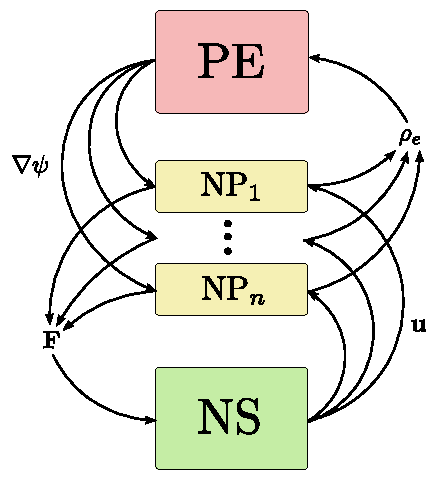
\includegraphics[width=0.5\textwidth]{fig/coupling.pdf}
\end{center}
\caption{Visualisation of the coupling between the three equations
  present in the model. Poisson's equation (PE), The set of
  Nernst-Planck equations (NP$_1$ ... NP$_n$) and the Navier-Stokes
  equations (NS). The dependencies have also be marked with arrows
  indicating what quantities for a certain equation that are needed
  from an other.}
\end{figure}


\section{The potential - Poisson's equation}\label{sec:et:poisson}
To be able to model the flow dynamics of liquids in a channel with
present EDLs, the potential and charge distribution
in the channel must be determined. These quantities are mutually
related through Poisson's equation for electrostatics:

\begin{equation}\label{eq:pb}
\nabla^2\psirm = -\frac{\rho_e}{\epsilon_r \epsilon_0}
\end{equation}
where $\psirm$ is the electrical potential, $\rho_e$ the electrical
charge density, $\epsilon_r$ is the relative permittivity and
$\epsilon_0$ the vacuum permittivity. Under certain assumptions, the
charge density may be explicitly determined as a function of the
potential distribution, one such result is the so called
Poisson-Boltzmann equation, further discussed in section \ref{sec:et:pb}.

\subsection{Boundary conditions}
At the charged boundaries, most physical situations may be covered by
either specifying the potential or the surface charge density. The
former would be a boundary condition of Dirichlet type:

\begin{equation}
\psirm(\x) = \zeta(\x)\;,\;\; \x \in \Gamma
\end{equation}
and the latter a boundary condition of Neumann type:

\begin{equation}\label{eq:et:fix_c}
\nabla\psirm(\x) \cdot \n =
-\frac{\sigma(\x)}{\epsilon_0\epsilon_r}\;,\;\; \x \in \Gamma
\end{equation}
where $\Gamma$ denotes the boundary of the domain and $\n$ is the
normal to the boundary surface.\- \cite{hlushkou}


\section{The transport of charges - Nernst-Planck equation}
The charge concentration in an electrolyte is indeed affected by its
environment. In the model proposed here, influences from: advection of
the electrolyte, diffusion due to concentration gradients and effects
from the electric field originating from charged objects placed at the
border or in the flow is considered. Charge conservation without any
external sources of the ion density, $\mathrm{C}(\x, t)$ gives:

\begin{equation}\label{eq:charge_conc}
\dfrac{\partial \C}{\partial t} + \nabla \cdot \J = 0
\end{equation}
where $\mathbf{J(\mathbf{x}, \mathrm{t})}$ is the net flux induced
by the effects described above. Explicit expressions for the fluxes
due to advection and diffusion respectively are 

\begin{equation}
\J_{adv} =
\C\ubf
\end{equation}
and 
\begin{equation}
\mathbf{J}_{dif} = -D\nabla \mathrm{C} 
\end{equation}
where $\mathbf{u}$ is the advective velocity and $D$ is the diffusion
coefficient. The ionic flux due to the presence of an electric
potential, $\psirm(\x, t)$, is given by the Nernst equation
\cite{dongquing-ren-book}:

\begin{equation}
\J_{ele} = -\frac{zq_eD}{k_BT}\C\nabla\psirm
\end{equation}
where $z$ is the relative charge of an ion, $q_e$ is the fundamental
charge, $k_B$ is the Boltzmann constant and $T$ is temperature of the
fluid.

Summing up the fluxes and putting them into eq. \eqref{eq:charge_conc} gives


\begin{equation}\label{np}
\dfrac{\partial \C}{\partial t} = \nabla \cdot \left [
 D\nabla \mathrm{C} - \C\ubf + \frac{zq_eD}{k_BT}\C\nabla\psirm
\right]
\end{equation}
which is a known result often referred to as the Nernst-Planck
equation. The advective velocity, $\ubf$, and the potential gradient,
$\nabla \psirm$, are obtained from couplings to the Navier-Stokes and
Poisson's equations respectively. More about the coupling between the
equations will be discussed in section \ref{et:coupling}.

\subsection{Boundary conditions}
Depending on the physical situation that is being modelled, different
conditions may be imposed at the boundaries of the domain. Throughout
this work, at hard boundaries (walls), the charge flux out of the
boundary will be set to zero, i.e.:

\begin{equation}
\J \cdot \mathbf{n}\big|_{x \in \Gamma} = 0 
\end{equation}
where $\mathbf{n}$ denotes the normal to the surface and $\Gamma$ is
the boundary of the domain. 


%what we need

%nernst planck


%poisson boltzmann steady state, fix potential 

\subsection{Poisson-Boltzmann equation}\label{sec:et:pb}
Consider a system consisting of an electrolyte in contact with a
(flat) charged wall.  Under certain assumptions, it is possible to
explicitly determine the charge density in eq. \eqref{np} as a
function of the electric potential. E.g. if there is no advection
present and if the system has reached a steady state, i.e. $\partial
\C /\partial t = 0$ and $\ubf = \mathbf{0}$ we have:

\begin{equation}\label{pb_constant_flux}
D\nabla \mathrm{C} + \frac{zq_eD}{k_BT}\C\nabla\psirm = \alpha
\end{equation} 
where $\alpha$ is some arbitrary constant. Due to the steady state
assumption, what the equation above actually says is that the net flux
of charge in the system is constant. Since no flux of charge is wanted
to flow through the wall boundary, the flux is set to zero on the wall
and since the flux is constant it will therefore be zero everywhere in
the liquid, i.e. $\alpha = 0$.

Considering only a one-dimensional situation with a position variable
$y$ varying in a direction out from the wall into the liquid,
eq. \eqref{pb_constant_flux} reads

\begin{equation}\label{eq:pb_eq_for_C}
\frac{1}{\C} \dfrac{d \C}{d y} + \frac{zq_e}{k_BT} \dfrac{d \psirm}{d
  y} = 0.
\end{equation}

The charge density is determined by solving eq. \eqref{eq:pb_eq_for_C}
for $\C$, i.e. integrating the equation. In order to avoid introducing
additional unknown quantities, the equation is integrated to far away
from the wall where the potential from the EDL is assumed to have
decreased to zero and where the concentrations, $\C^{\infty}$, of the
electrolyte is known.

\begin{equation}
\int_y^{\infty} d\ln( \C(y')) = -\frac{z q_e}{k_BT}\int_y^{\infty}d\psirm(y')
\end{equation}
This gives an expression for $C(y)$:

\begin{equation}\label{eq:C}
\C(y) = \C^{\infty} \exp\left(-\frac{z q_e \psirm(y)}{k_BT}\right).
\end{equation}

In a general case, there may be several species of ions in the
electrolyte, the net charge density, $\rho_e$, is then given by simply
summing up the contributions from the different species:

\begin{equation}\label{eq:rho}
\rho_e = q_e\sum_i z_i \C_i.
\end{equation}

Summarising eqs. \eqref{eq:pb}, \eqref{eq:C} and \eqref{eq:rho} gives
the Poisson-Boltzmann equation in one dimension

\begin{equation}\label{eq:pb_real}
\dfrac{d^2\psirm(y)}{dy^2} = -\frac{q_e}{\epsilon_r \epsilon_0}\sum_i z_i
\C_i^{\infty} \exp\left(-\frac{z_i q_e \psirm(y)}{k_BT}\right).
\end{equation}

\subsubsection{The Debye–Hückel approximation}
Historically, the non-linear nature of eq. \eqref{eq:pb_real}
complicated when it came to solving it. This was a major difficulty in
the past when the computational power at hands were rather limited. A
linearisation is therefore sometimes done, this linear version of the
PB equation is often referred to as the Debye–Hückel
approximation. The solution of the linearisation gives however,
something to compare with and will be used when defining a
characteristic length scale of the EDL.

For a 1:1 electrolyte solution, eq. \eqref{eq:pb_real} reduces to

\begin{equation}
\frac{d^2\psi(x)}{dx^2} = \frac{2n^{\infty}q_ez}{\epsilon_r
  \epsilon_0}
\sinh\left(\frac{z q_e \psi(x)}{k_BT}\right).
\end{equation}
and the linearised equation is

\begin{equation}
\frac{d^2\psi(x)}{dx^2} = \frac{2n^{\infty}q_e^2z^2}{\epsilon_r
  \epsilon_0 k_B T} \psi(x) = \kappa^2 \psi(x)
\end{equation}
where $\kappa^{-1}$ is the Debye length and gives a measure for the
characteristic size of the EDL.

\subsubsection{Limitations of the Poisson-Boltzmann model}
As the Poisson-Boltzmann equation is derived several assumptions are
made. First, the net flux of ions are assumed to be zero and that the
advective contribution the flux is negligible. Thus, the PB equation is
only applicable when the system is at (or very close) thermodynamical
equilibrium.

\todo{Continue this discussion...}


%% In this work, flows of ionic solution will be studied and the
%% assumption with thermodynamical equilibrium does not apply. However
%% for low-speed flows the model may still be a decent approximation,
%% which will be investigated.

%% The second assumption, may also stay unfulfilled in some cases
%% investigated here. The fluid in contact with the wall must be of
%% substantial size in relation to the EDL thickness. There will be
%% cases where the choice of $\zeta$ potential in combination with thin
%% channels will make this assumption not fulfilled.

%% Since the PB equation is unable to model the system of
%% interest, a different approach will be presented. However, throughout
%% this work, references and comparisons with the PB model w
%% ill be made. 


%intro

%liten härledning av högerledet 
%diffusion by conc grad. = grad of
%potential <==> termodynamic equilibrium
%chem pot definerad som....
% eq.
% boundary conditions
%antagaganden !!!


%% A simple and commonly used approach for determining potentials (and
%% charge distributions) in systems with present EDLs is by solving
%% eq. \eqref{eq:pb} with a charge distribution of Boltzmann
%% type. Here follows a brief derivation of this term together with some
%% discussion on the assumptions made.

%% The fundamental assumption that the derivation of the charge
%% distribution is based on, is the fact that the system is assumed to be
%% under thermodynamical equilibrium. I.e. forces, acting on the ions,
%% due to chemical diffusion from concentration gradients and from the
%% electrical field are therefore balancing each other. In one dimension:

%% \begin{equation}\label{eq:dif_elec_forces}
%% \frac{d \mu_i}{dx} = -z_i q_e\frac{d\psi}{dx}
%% \end{equation}
%% where $\mu_i$ is the chemical potential for species $i$, $z_i$ is the
%% relative charge of species $i$, $q_e$ the fundamental charge and
%% $\psi$ is the EDL potential. The chemical potential is given by
%% \cite{ren}:

%% \begin{equation}
%% \mu_i = \mu_i^{\infty} + k_BT\ln n_i
%% \end{equation}
%% where $\mu_i^{\infty}$ is a reference value for the chemical potential,
%% here the potential value far from the charged wall is used, $k_BT$ is
%% the thermal energy and $n_i$ is the ion concentration of species
%% $i$. This expression plugged into eq. \eqref{eq:dif_elec_forces} gives

%% \begin{equation}\label{eq:eq_for_ni}
%% \frac{d \ln(n_i)}{dx} = - \frac{z_i q_e}{k_BT}\frac{d \psi}{dx}.
%% \end{equation}


\section{The velocity field - Navier-Stokes equations}\label{sec:et:ns}
In hydrodynamics, the Navier-Stokes equations are one of the most
fundamental corner stones. They describe the motion of a fluid under
the influence of various internal and external forces. 

For later convenience and for reference when it comes to deriving the
Lattice-Boltzmann formulation of the NS equation, a brief sketch of a
derivation will here be presented. A most general form of the
Navier-Stokes equation follows from momentum conservation

\begin{equation}
\dfrac{\partial (\rhorm \ubf)}{\partial t} + \nabla \cdot (\rho \ubf
\otimes \ubf) + \Q = 0 
\end{equation}
where, $\rhorm$ is fluid density, $\ubf$ is velocity and $\Q$ is a
momentum source term (force per volume). Expanding the time
derivative and the divergence terms respectively gives
 
\begin{equation}\label{eq:et:nspre}
\ubf \left ( \dfrac{\partial \rhorm}{\partial t} + \nabla \cdot
  (\rhorm \ubf) \right ) + \rhorm \left (\dfrac{\partial \ubf}{\partial t} +
  \ubf \cdot \nabla \ubf 
  \right ) + \Q = 0.
\end{equation}
By assuring mass conservation (without sources) we have that

\begin{equation}\label{eq:et:mass_conc}
 \dfrac{\partial \rhorm}{\partial t} + \nabla \cdot(
  \rhorm \ubf) = 0
\end{equation}
and eq. \eqref{eq:et:nspre} reduces to

\begin{equation}\label{eq:et:ns_general} 
\rhorm \left (\dfrac{\partial \ubf}{\partial t} +
  \ubf \cdot \nabla \ubf 
  \right ) + \Q = 0
\end{equation}
which together with eq. \eqref{eq:et:mass_conc} is a general
formulation of the Navier stokes equations. 

The force term $\Q$, is determined by the physical properties of the
fluid and from its environment. In this work, only incompressible
Newtonian fluids will be studied. The force contribution to $\Q$
involved in that case is limited to viscous forces, pressure gradients
in the fluid and to external force fields. Putting that into
eqs. \eqref{eq:et:mass_conc} and \eqref{eq:et:ns_general} gives

\begin{equation}\label{eq:et:ns_incompressible}
 \nabla \cdot \ubf = 0
\end{equation}
and

\begin{equation}\label{eq:et:ns_mom}
\rhorm \left (\dfrac{\partial \ubf}{\partial t} +
  \ubf \cdot \nabla \ubf 
  \right ) = - \nabla \Prm  + \mu \nabla^2 \ubf + \F
\end{equation}
where $\Prm$ is the pressure, $\mu$ the kinematic viscosity and $\F$
is the contributions from  external forces.

\subsection{Boundary conditions}

At hard boundaries (walls), the boundary conditions to
eqs. \eqref{eq:et:ns_incompressible} and \eqref{eq:et:ns_mom} are set
on the velocity of either a Dirichlet or Neumann type. In most
physical situations the Dirichlet condition is used which corresponds
to that there is a friction between the fluid and the wall, usually
full friction, i.e. when no relative movement between fluid and wall
is present and the velocity at the wall boundary is set to zero, i.e.

\begin{equation}
\ubf = 0 \;,\;\; \x \in \Gamma
\end{equation} 
where $\Gamma$ denotes the boundary. The Neumann type conditions are
used for no-friction walls where the normal component of the
derivative of the velocity is specified, usually to zero.

At wet boundaries, inlets and outlets, of the domain various boundary
conditions may be set. For instance the pressure or the velocity could
be fixed. In the case of a fixed pressure boundary, a flow direction
must also be specified for completeness. \cite{some fluid dynamics
  text}


\section{Pressure-driven electrokinetic flow}\label{sec:et:streaming_pot}
As a charged fluid is driven by a pressure gradient, a movement of
charges, i.e. an electrical current will be induced. Due to the charge
flux, a potential gradient will build up along the flow
direction. This potential is usually referred to as the streaming
potential, $\phi(\x)$, and its magnitude is determined from the
induced current through Ohm's law

\begin{equation}
\J = -  \sigma \nabla \phi  
\end{equation}   
where $\sigma$ is the conductivity of the fluid. in a perfectly
conducting fluid there will be no potential differences. Also a
complete neutral solution will carry no net current and also in this
case there will be no potential differences.

Charges under the influence of an electric field will be affected by a
force. Charges moving due to this force will, in a liquid, also pull
liquid (uncharged) molecules with them. In a macroscopic limit, the
force density affecting the charges in the liquid is assumed to affect
the liquid as a whole. The volumetric force affecting the fluid from
the presence of the streaming potential is then given by:

\begin{equation}
\F = - \rho_e \nabla \phi
\end{equation}
where $\rho_e$ is the charge density. This is an example of how the
charge density from the Nernst-Planck equation may couple to the force
term in Navier-Stokes equations. 

This force will always be affecting the fluid in a direction opposite
to the net flux of charge, i.e. the force will slow the fluid down,
this is illustrated in fig. \ref{fig:et:ev}. This effect that a moving
net charged fluid is slowed down is called the \emph{electroviscous
  effect}. The name originates from that a similar effect might be
achieved by increasing the viscosity of the fluid.

\begin{figure}
\begin{center}
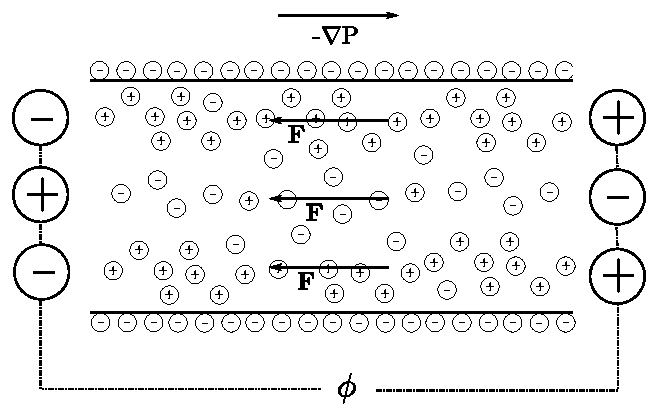
\includegraphics[width=0.7\textwidth]{fig/channel_electroviscous.pdf}
\end{center}
\caption{Example of an electroviscous system. The fluid is driven by a
  pressure gradient, $\nabla \Prm$. The directions of the forces on
  the fluid are always opposite to the flow direction. The force
  originates from the potential difference, $\phi$, that builds up
  along the channel. The force is always opposite to the flow
  direction, thus slowing the flow down.}
\label{fig:et:ev}
\end{figure}


\section{Electroosmotic flow}\label{sec:et:electroosmosis}
Instead of driving the fluid flow through a pressure drop, a net
charged fluid may be driven by an external electric field. This may
be seen as the opposite case to that in section
\ref{sec:et:streaming_pot} where a current is induced by a pressure
drop.

The volumetric force on the fluid from the external field, $\E_{ext}$,
is given by

\begin{equation}
\F = \rhorm_e \E_{ext}
\end{equation}

where $\rho_e$ is the charge density. If the electric field is
constant (or at least has the same direction) everywhere, the sign of
the force is not in the same direction for a net charged positive area
of the fluid as for a net charged negative. Thus the fluid may be
either slowed down or sped up. This is a qualitative difference to
pressure driven situation and is illustrated in fig. \ref{fig:et:eo}.

\begin{figure}
\begin{center}
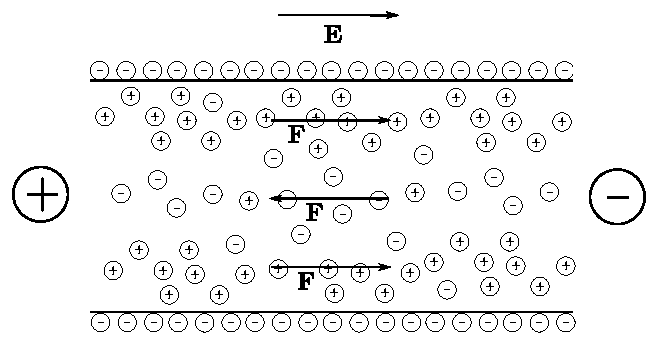
\includegraphics[width=0.7\textwidth]{fig/channel_electroosmosis.pdf}
\end{center}
\caption{Example of an electroosmotic system. The fluid is driven by
  an external electric field, $\E$. The directions of the forces on
  the fluid from the electric field are indicated with arrows. Note
  however that the fluid does not necessarily has to flow in the
  direction of the force, this due to viscous effects in the fluid. }
\label{fig:et:eo}
\end{figure}

The electroviscous effect is in the case of pure electroosmotic flow
usually neglected as the field due to the streaming potential is, in
most physical cases, small in comparison to the applied external
field. \cite{wang-poi}


%lite intro

%börja inte med allmän teoretisk formulering

%sedan lite resultat, double layers

%pressure driven flows...
